% -*- mode: LaTeX; TeX-PDF-mode: t; -*- 
% LaTeX path to the root directory of the current project
% from the directory in which this file resides
% and path to econtexPaths which defines the rest of the paths like \FigDir
\providecommand{\econtexRoot}{}\renewcommand{\econtexRoot}{.}
\providecommand{\econtexPaths}{}\renewcommand{\econtexPaths}{econtexPaths}
% -*- mode: LaTeX; TeX-PDF-mode: t; -*- 
% The \commands below are required to allow sharing of the same base code via Github between TeXLive on a local machine and Overleaf (which is a proxy for "a standard distribution of LaTeX").  This is an ugly solution to the requirement that custom LaTeX packages be accessible, and that Overleaf prohibits symbolic links
\providecommand{\packages}{\econtexRoot/Resources/texmf-local/tex/latex}
\providecommand{\econtex}{\packages/econtex}
\providecommand{\econark}{\econtexRoot/Resources/texmf-local/tex/latex/econark}
\providecommand{\econtexSetup}{\econtexRoot/Resources/texmf-local/tex/latex/econtexSetup}
\providecommand{\econarkSetup}{\econtexRoot/Resources/texmf-local/tex/latex/econarkSetup}
\providecommand{\econtexShortcuts}{\econtexRoot/Resources/texmf-local/tex/latex/econtexShortcuts}
\providecommand{\econtexBibMake}{\econtexRoot/Resources/texmf-local/tex/latex/econtexBibMake}
\providecommand{\econtexBibStyle}{\econtexRoot/Resources/texmf-local/bibtex/bst/econtex}
\providecommand{\econtexBib}{economics}
\providecommand{\notes}{\econtexRoot/Resources/texmf-local/tex/latex/handout}
\providecommand{\handoutSetup}{\econtexRoot/Resources/texmf-local/tex/latex/handoutSetup}
\providecommand{\handoutShortcuts}{\econtexRoot/Resources/texmf-local/tex/latex/handoutShortcuts}
\providecommand{\handoutBibMake}{\econtexRoot/Resources/texmf-local/tex/latex/handoutBibMake}
\providecommand{\handoutBibStyle}{\econtexRoot/Resources/texmf-local/bibtex/bst/handout}

\providecommand{\FigDir}{\econtexRoot/Figures}
\providecommand{\CodeDir}{\econtexRoot/Code}
\providecommand{\DataDir}{\econtexRoot/Data}
\providecommand{\SlideDir}{\econtexRoot/Slides}
\providecommand{\TableDir}{\econtexRoot/Tables}
\providecommand{\ApndxDir}{\econtexRoot/Appendices}

\providecommand{\ResourcesDir}{\econtexRoot/Resources}
\providecommand{\rootFromOut}{..} % APFach back to root directory from output-directory
\providecommand{\LaTeXGenerated}{\econtexRoot/LaTeX} % Put generated files in subdirectory
\providecommand{\econtexPaths}{\econtexRoot/Resources/econtexPaths}
\providecommand{\LaTeXInputs}{\econtexRoot/Resources/LaTeXInputs}
\providecommand{\LtxDir}{LaTeX/}
\providecommand{\EqDir}{\econtexRoot/Equations} % Put generated files in subdirectory

\providecommand{\titlepagecustom}{\LaTeXInputs/titlepagecustom}


\documentclass[\econtexRoot/HAFiscal]{subfiles}
\onlyinsubfile{\externaldocument{\econtexRoot/HAFiscal}} % Get xrefs -- esp to apndx -- from main file; only works if main file has already been compiled

\begin{document}

\addcontentsline{toc}{section}{Appendices} % label the section "Appendices"

\hypertarget{Appendices}{} % Allows link to [url-of-paper]#Appendices
\ifthenelse{\boolean{Web}}{}{% Web version has no page headers
  \chead[Appendices]{Appendices}      % but PDF version does
  \appendixpage % Reset formatting for appendices
} 

%\hypertarget{Estimating-discount-factor-distributions-for-different-interest-rates}{}\par\section{Estimating discount factor distributions for different interest rates}
%\notinsubfile{\label{app:DF_R}}
%
%
%
%Figure~\ref{fig:LorenzPtsrobustnessR} shows the fit of the liquid wealth distribution for interest rates of $0.5$ percent and $1.5$ percent per quarter. In both cases, the estimation exactly matches the median liquid wealth to permanent income ratios for each education group listed in Panel~B of Table~\ref{tab:estimBetas}. 
%
% \begin{table}{th}
%   \begin{center}
%     \begin{tabular}{lccc}
%        %         \multicolumn{4}{l}{Panel (B) Estimation targets} \\ \midrule
%        %         & Dropout & Highschool & College \\ \midrule
%        %         Median LW/PI (data) & 4.64 & 30.2 & 112.8 \\ 
%        %         Median LW/PI (model, $R = 1.005$) & 4.64 & 30.2 & 112.8 \\	
%        %         Median LW/PI (model, $R = 1.01$) & 4.64 & 30.2 & 112.8 \\
%        %         Median LW/PI (model, $R = 1.015$) & 4.64 & 30.2 & 112.8 \\ \bottomrule
%        %       \end{tabular} \\ \\ 
%        %         \end{center}	
%        %         \end{table}
%
%\begin{figure}[th]
%  \begin{center}
%    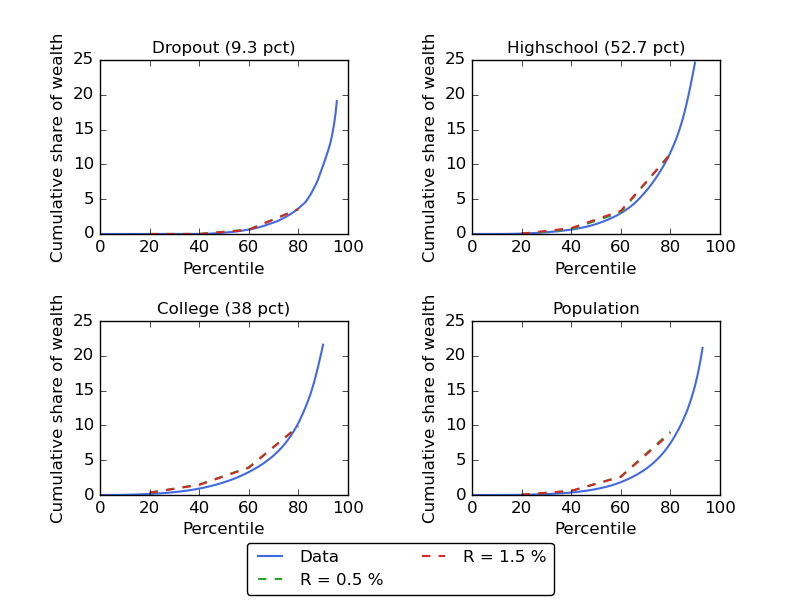
\includegraphics[width=.9\textwidth]{\econtexRoot/Figures/LorenzPoints_robustness_R}
%    \caption{Distributions of liquid wealth within each educational group and for the whole population from the 2004 Survey of Consumer Finance and from the estimated model for different values of the interest rate, $R$.}
%    \notinsubfile{\label{fig:LorenzPtsrobustnessR}}
%  \end{center}
%\end{figure}
%
%
%
%\FloatBarrier


%\subfile{Robustness}
% -*- mode: LaTeX; TeX-PDF-mode: t; -*- 
% LaTeX path to the root directory of the current project
% from the directory in which this file resides
% and path to econtexPaths which defines the rest of the paths like \FigDir
\providecommand{\econtexRoot}{}\renewcommand{\econtexRoot}{.}
\providecommand{\econtexPaths}{}\renewcommand{\econtexPaths}{econtexPaths}
% -*- mode: LaTeX; TeX-PDF-mode: t; -*- 
% The \commands below are required to allow sharing of the same base code via Github between TeXLive on a local machine and Overleaf (which is a proxy for "a standard distribution of LaTeX").  This is an ugly solution to the requirement that custom LaTeX packages be accessible, and that Overleaf prohibits symbolic links
\providecommand{\packages}{\econtexRoot/Resources/texmf-local/tex/latex}
\providecommand{\econtex}{\packages/econtex}
\providecommand{\econark}{\econtexRoot/Resources/texmf-local/tex/latex/econark}
\providecommand{\econtexSetup}{\econtexRoot/Resources/texmf-local/tex/latex/econtexSetup}
\providecommand{\econarkSetup}{\econtexRoot/Resources/texmf-local/tex/latex/econarkSetup}
\providecommand{\econtexShortcuts}{\econtexRoot/Resources/texmf-local/tex/latex/econtexShortcuts}
\providecommand{\econtexBibMake}{\econtexRoot/Resources/texmf-local/tex/latex/econtexBibMake}
\providecommand{\econtexBibStyle}{\econtexRoot/Resources/texmf-local/bibtex/bst/econtex}
\providecommand{\econtexBib}{economics}
\providecommand{\notes}{\econtexRoot/Resources/texmf-local/tex/latex/handout}
\providecommand{\handoutSetup}{\econtexRoot/Resources/texmf-local/tex/latex/handoutSetup}
\providecommand{\handoutShortcuts}{\econtexRoot/Resources/texmf-local/tex/latex/handoutShortcuts}
\providecommand{\handoutBibMake}{\econtexRoot/Resources/texmf-local/tex/latex/handoutBibMake}
\providecommand{\handoutBibStyle}{\econtexRoot/Resources/texmf-local/bibtex/bst/handout}

\providecommand{\FigDir}{\econtexRoot/Figures}
\providecommand{\CodeDir}{\econtexRoot/Code}
\providecommand{\DataDir}{\econtexRoot/Data}
\providecommand{\SlideDir}{\econtexRoot/Slides}
\providecommand{\TableDir}{\econtexRoot/Tables}
\providecommand{\ApndxDir}{\econtexRoot/Appendices}

\providecommand{\ResourcesDir}{\econtexRoot/Resources}
\providecommand{\rootFromOut}{..} % APFach back to root directory from output-directory
\providecommand{\LaTeXGenerated}{\econtexRoot/LaTeX} % Put generated files in subdirectory
\providecommand{\econtexPaths}{\econtexRoot/Resources/econtexPaths}
\providecommand{\LaTeXInputs}{\econtexRoot/Resources/LaTeXInputs}
\providecommand{\LtxDir}{LaTeX/}
\providecommand{\EqDir}{\econtexRoot/Equations} % Put generated files in subdirectory

\providecommand{\titlepagecustom}{\LaTeXInputs/titlepagecustom}


\documentclass[\econtexRoot/HAFiscal]{subfiles}
\onlyinsubfile{\externaldocument{\econtexRoot/HAFiscal}} % Get xrefs -- esp to apndx -- from main file; only works if main file has already been compiled

\begin{document}
	
\FloatBarrier
\hypertarget{hank_appendix}{}\par\section{Details of the HANK and SAM Model}
\notinsubfile{\label{sec:hank_appendix}}


\subsection{Households}

The household block follows closely to the main text with a few exceptions. First, the splurge only occurs out of equilibrium---that is, the steady state of the model is calculated without the splurge behavior. Second, the level of permanent income of all newborns is equal to one. Furthermore, all households face the same employment to unemployment and unemployment to employment probabilities. The probabilities are calibrated to the transition probabilities of high school graduates from the main text. Lastly, following the notation of \cite{Auclert2020}, $r^{a}_{t}$ will denote the economy wide ex-ante real interest rate.


\subsection{Goods Market}

A continuum of monopolistically competitive intermediate goods producers, indexed by \( j \in [0,1] \), produces intermediate goods \( Y_{jt} \), which are sold to a final goods producer at price \( P_{jt} \). Each period, these producers fully consume their profits.


\subsubsection{Final Goods Producer}

A perfectly competitive final goods producer purchases intermediate goods \( Y_{jt} \) from intermediate good producer $j$ at price \( P_{jt} \) and produces the final good \( Y_t \) using a CES production function:

$$ Y_{t} = \left(\int_{0}^{1} Y_{jt}^{\frac{\epsilon_{p}-1}{\epsilon_{p}}}\, dj\right)^{\frac{\epsilon_{p}}{\epsilon_{p}-1}},$$ 
where $\epsilon_{p}$ is the elasticity of substitution.

Given $P_{jt}$, the price of intermediate good $j$, the final goods producer maximizes profits by solving:
$$ \max_{Y_{jt}} P_{t} \left(\int_{0}^{1} Y_{jt}^{\frac{\epsilon_{p}-1}{\epsilon_{p}}}\, dj\right)^{\frac{\epsilon_{p}}{\epsilon_{p}-1}} - \int_{0}^{1} P_{jt} Y_{jt} ,\ dj.$$ 
%\vspace{.2cm}

The first order condition leads to demand for good $j$ given by
$$Y_{jt} = \left(\frac {P_{jt}}{P_{t}}\right)^{- \epsilon_{p}} Y_{t},$$
and the price index
$$P_{t} = \left(\int_{0}^{1} P_{jt}^{1-\epsilon_{p}}\,dj \right )^{\frac{1}{1-\epsilon_{p}}}.$$


\subsubsection{Intermediate Goods Producers}

Intermediate goods producers produce according to a production function linear in labor~$L_{t}$: 
$$Y_{jt} =  Z L_{jt},$$ 
where $Z$ is total factor productivity.
%\vspace{.3cm}
  
Each intermediate goods producer hires labor \( L_t \) from a labor agency at cost \( h_t \). Given this labor cost, each producer sets \( P_{jt} \) to maximize profits while facing price stickiness à la \cite{Rotemberg1982}. In HANK models with sticky prices, profits tend to be countercyclical, and when households have high MPCs, this can generate countercyclical consumption responses to dividends. To simplify, we assume that intermediate goods producers fully consume their profits rather than distributing them to households, thereby abstracting from consumption responses to firm profits. Each producer maximizes profits by solving:

$$J_{t}\left(P_{jt}\right) = \max_{\{P_{jt}\}} \left\{\frac{P_{jt}Y_{jt}}{P_{t}} - h_{t} L_{jt} -  \frac{\varphi}{2}\left( \frac{P_{jt} - P_{jt-1}}{P_{jt-1}} \right)^{2} Y_{t}  + J_{t+1}\left(P_{jt+1}\right) \right\},$$ 

where $\varphi$ determines the cost of adjusting the price and, hence, the degree of price stickiness. 

The problem can be rewritten as the standard New Keynesian maximization problem:
$$\max_{\{P_{jt}\}} \mathrm{E}_{t}\left[\sum_{s=0}^{\infty}  M_{t,t+s} \left( \left( \frac{P_{jt+s}}{P_{t+s}} - MC_{t+s}\right)Y_{jt+s} -  \frac{\varphi}{2}\left( \frac{P_{jt+s}}{P_{jt+s-1}} - 1\right)^{2} Y_{t+s} \right)\right],$$ 
where $MC_{t} = \frac{h_{t}}{Z}$.

Given that all firms face the same adjustment costs, there exists a symmetric equilibrium where all firms choose the same price with $P_{jt}=P_{t}$ and $Y_{jt}=Y_{t}$.

The resulting Phillips Curve is
$$ \epsilon_{p} MC_{t} = \epsilon_{p} - 1 + \varphi ( \Pi_{t} -1) \Pi_{t} - M_{t,t+1} \varphi (\Pi_{t+1} -1 ) \Pi_{t+1} \frac{Y_{t+1}}{Y_{t}}$$
where $\Pi_{t} = \frac{P_{t}}{P_{t+1}}$. 

\subsection{Labor market}

A risk-neutral labor agency supplies labor \( N_t \) to intermediate goods producers at cost \( h_t \) by hiring households at wage \( w_t \). To hire workers, the agency posts vacancies \( v_t \), which are filled with probability \( \phi_t \). Household job search is random. Following \cite{Bardoczy2022}, we assume the labor agency cannot observe individual household productivity. Instead, it only observes the average productivity of all employed workers, which is normalized to one.


\textbf{Labor agency.} The labor agency determines how many vacancies to post and how much labor to sell by solving the following problem: 
$$J_{t}(N_{t-1})  = \max_{N_{t},v_{t}} \left\{( h_{t} - w_{t}) N_{t}- \kappa v_{t} + \mathrm{E_{t}}\left[ \frac{J_{t+1}(N_{t})}{1 + r^{a}_{t}}\right]\right\},$$
subject to
$$ N_{t} = (1-\omega)N_{t-1} + \phi_{t} v_{t}.$$ 

The parameters $\kappa$ and $\omega$ are, respectively, the cost of posting a vacancy, and the job separation rate. 

The resulting job creation curve is:
$$ \frac{\kappa}{\phi_{t}}  = (h_{t} - w_{t})+  (1-\omega)\mathrm{E_{t}}\left[   \frac{\kappa}{(1+r^{a}_{t}) \phi_{t+1}} \right].$$

\textbf{Matching.} The matching process between households and the labor agency follows a Cobb-Douglas matching function:
$$m_{t} = \chi e_{t}^{\alpha} v_{t}^{1-\alpha},$$ 
where $m_{t}$ is the mass of matches, $e_{t}$ is the mass of job searchers, $\alpha$ is the matching function elasticity, and $\chi$ is a matching efficiency parameter.

The vacancy filling probability \( \phi_t \) and the job finding probability \( \eta_t \) evolve as follows:
$$\eta_{t} = \chi \Theta_{it}^{1-\alpha} $$
%$$\eta_{t}(X) = \chi q(X) \Theta_{it}^{1-\alpha} $$
$$ \phi_{t} = \chi \Theta_{t}^{-\alpha} $$ 
where $\Theta_{t} = \frac{v_{t}}{e_{t}}$ is labor market tightness.

\textbf{Wage Determination.} Following \cite{Gornemann2021} and \cite{Blanchard2010}, we assume the real wage evolves according to the following rule:
$$log\left(\frac{w_{t}}{w_{ss}}\right)  = \phi_w log\left( \frac{ w_{t-1}}{ w_{ss}} \right) +   (1 - \phi_w) log\left( \frac{N_{t}}{N_{ss}}\right),$$
where $\phi_w$ dictates the extent of real wage rigidity. 

\subsection{Fiscal Policy}

The government issues long term bonds $B_{t}$ at price $q^{b}_{t}$ in period $t$ that pays $\delta^{s}$ in period $t+s+1$ for $s \in \{0,1,2,\ldots\}$.

The bond price satisfies the no arbitrage condition:
$$q^{b}_{t} = \frac{ 1  + \delta \mathrm{E}_{t}[q^{b}_{t+1}]}{1+r^{a}_{t}}.$$ 

The government funds its expenditures through debt and taxes, subject to the following budget constraint:
$$ (1 + \delta q^{b}_{t})B_{t-1} + G_{t}  + S_{t} = \tau_{t} w_{t} N_{t}+ q^{b}_{t}B_{t},$$
where $S_{t}$ are payments for unemployment insurance and other transfers.

For all stimulus policies, except tax cuts, we follow \cite{Auclert2020} and allow the tax rate to adjust in order to stabilize the debt-to-GDP ratio:
$$\tau_{t} - \tau_{ss} = \phi_{B} q^{b}_{ss} \frac{B_{t-1} - B_{ss} }{Y_{ss}}$$
where $\phi_{B}$ governs the speed of adjustment. 

For the tax cuts, we assume government expenditures adjust following:
$$G_{t} - G_{ss} = \phi_{G} q^{b}_{ss} \frac{B_{t-1} - B_{ss} }{Y_{ss}}$$
where $\phi_{G}$ governs the speed of adjustment of government spending in response to debt. 

\subsection{Monetary Policy}

The central bank follows a standard Taylor rule that responds solely to inflation:
$$i_{t} = r^{*} +\phi_{\pi} \pi_{t},$$ 
where $\phi_{\pi}$ is the coefficient on inflation. Inflation is given by $\pi_t = P_t/P_{t-1}-1$, and~$r^{*}$ is the steady state interest rate. 

\subsection{Equilibrium}

An equilibrium in this economy is a sequence of: 
\begin{itemize}[label=--]
	\item Policy Functions $\left( c_{it}(m) \right )_{t=0}^{\infty}$ normalized by permanent income.
	\item Prices $ \left( r^{a}_{t+1}, i_{t}, q^{b}_{t},  w_{t}, h_{t} , \pi_{t} , \tau_{t} \right) _{t=0}^{\infty}$.
	\item Aggregates $ \left(C_{t}, Y_{t} , N_{t},   \Theta_{t},  B_{t} , A_{t}  \right)_{t=0}^{\infty}$.
\end{itemize}

Such that: 
\begin{itemize}[label=--]
\item $\left(c_{it}(m)\right)_{t=0}^{\infty}$  solves the household's maximization problem given $\left( w_{t}, \eta_{t},  r^{a}_{t} , \tau_{t} \right)_{t=0}^{\infty}$.
\item The final goods producer and intermediate goods producers both maximize their respective objective functions.
\item The nominal interest rate is determined by the central bank's Taylor rule.
\item The tax rate is set according to the fiscal rule, ensuring that the government budget constraint is satisfied.
\item The value of assets is equal to the value of government bonds:
 $$A_t =  q^{b}_{t}B_{t}.$$
\item The goods market clears\footnote{Note if profits were not held by firms then the goods market condition would be $ C_{t}  + G_{t}  = Y_{t} -  \kappa v_{t} - \frac{\varphi}{2}\left( \frac{P_{t}}{P_{t-1}} - 1\right)^{2} Y_{t}  $.  In particular, since firm profits are $D_{t} = Y_{t} -  w_{t} N_{t}  - \kappa v_{t} - \frac{\varphi}{2}\left( \frac{P_{t}}{P_{t-1}} - 1\right)^{2} Y_{t} $, then the goods market condition would become $ C_{t}  + G_{t}  =w_{t} N_{t}  + D_{t} = Y_{t} -  \kappa v_{t} - \frac{\varphi}{2}\left( \frac{P_{t}}{P_{t-1}} - 1\right)^{2} Y_{t}  $. }: 
$$ C_{t}  = w_{t} N_{t}  + G_{t},$$
where $C_{t} \equiv  \int_{0}^{1} \textbf{c}_{it} \, di$. 
\item The labor demand of intermediate goods producers equals labor supply of labor agency:
$$ L_{t} =  N_{t}.$$ 
\end{itemize}

%\input{\TableDir/Calibration.tex}


\begin{table}
\begin{center}
\renewcommand{\arraystretch}{1.6}
\caption{Calibration}\label{table:Calibration}
\makebox[\textwidth]{\begin{tabular}{l c c l}
Description & Parameter & Value & Source/Target \\ \hline
Elasticity of Substitution & $\epsilon_{p}$ & 6 & Standard \\
Price Adjustment Costs & $\varphi$ & 96.9 & \cite{Ravn2017} \\
Vacancy Cost & $\kappa$ & 0.056 & $\frac{\kappa}{w\phi} = 0.071$ \\
Job Separation Rate & $\omega$ & 0.092 & Match $\pi(eu)$ for Highschool group \\
Matching Elasticity & $\alpha$ & 0.65 & \cite{Ravn2017} \\
Job Finding Probability & $\eta_{ss}$ & 0.67 & $\pi(ue)$ in section~\ref{sec:calib} \\
Vacancy Filling Rate & $\phi_{ss}$ & 0.71 & den Haan et al. (\citeyear{DenHaan2000}) \\
Real Wage Rigidity parameter & $\phi_{w}$ & 0.837 & Gornemann et al. (\citeyear{Gornemann2021}) \\
Government Spending & $G$ & 0.38 & Gov. budget constraint \\
Decay rate of Gov. Coupons & $\delta$ & 0.95 & 5 Year Maturity of Debt \\
Response of Tax Rate to Debt & $\phi_{B}$ & 0.015 & Auclert et al. (\citeyear{Auclert2020}) \\
Taylor Rule Inflation Coefficient & $\phi_{\pi}$ & 1.5 & Standard \\ \hline
\end{tabular}}
\end{center}
\end{table}

\section{Calibration of Non-Household Blocks }

The elasticity of substitution is set to 6, and the price adjustment cost parameter is set to 96.9 as in \cite{Ravn2017}.
The vacancy cost is set to 7\% of the real wage as in \cite{Christiano2016}.\footnote{The range of plausible values lie between $4\%$ and $14\%$ \cite{Silva2009}} The matching elasticity is 0.65 following \cite{Ravn2017}. The job separation rate is set to 0.092. As in section~\ref{sec:calib}, we set the job finding probability in the steady state for the unemployed $\eta_{ss}$ to 0.67. Along with the job separation rate, this gives a probability of transitioning from employment to unemployment within a quarter of $3.1$ percent which is the value we use for the Highschool group in section~\ref{sec:calib}. The quarterly vacancy filling rate is 0.71 as in \cite{DenHaan2000} (and together with our other choices, this pins down the matching efficiency $\chi$). The degree of wage rigidity $\phi_w$ is set to 0.837 following \cite{Gornemann2021}. The tax rate is set to 0.3 and government spending is set to clear the government budget constraint. The parameters that dictate the speed of fiscal adjustment, $\phi_{B}$ and $\phi_{G}$, are set to 0.015, the lower bound of the estimates in \cite{Auclert2020}.\footnote{The speed of adjustment parameter is set to the lower bound to ensure that the policies evaluated in the HANK and SAM model are almost entirely deficit financed.} Furthermore, the decay rate of government coupons is set to $\delta = 0.95$ to match a maturity of 5 years.\footnote{The duration of bonds in the model is $\frac{(1+r)^4}{(1+r)^4 - \delta}$} Finally, the Taylor rule coefficient on inflation is set to the standard value of $\phi_{\pi}=1.5$. 


\ifthenelse{\boolean{Web}}{}{
\end{document} \endinput
}



\ifthenelse{\boolean{Web}}{}{
\end{document} \endinput
}

ut_splurge}}

In this appendix, we consider the implications for our results of removing splurge consumption from the model.
First, we discuss that model's ability to match the empirical targets that we used to estimate the splurge in section~\ref{sec:splurge}.
Second, we repeat the estimation of discount factor distributions in the US model in section~\ref{sec:estimBetas}, and discuss the implications for both targeted and untargeted moments.
Finally, we use the reestimated model to asses the relevance of the splurge for the effectiveness of the three policies.


\subsection{Matching the iMPCs without the splurge}
%{Estimating discount factor distributions in the absence of the splurge}

For the purpose of evaluating the results in the model without the splurge we do not require the reestimation of our Norwegian model, as the purpose of the latter is the estimation of the splurge.
Nevertheless, we test how well the model can match the dynamics of spending after a temporary income shock as reported by \citet{fagereng_mpc_2021} when the splurge is zero.
Figure~\ref{fig:splurge0_Norwayestimation} illustrates the fit without the splurge and compares it to our baseline estimation.


\begin{figure}[htb]
	\centering
	\begin{subfigure}[b]{.48\linewidth}
		\centering
		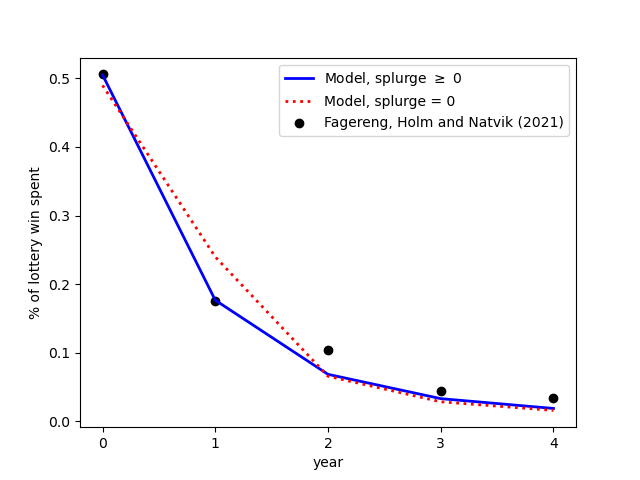
\includegraphics[width=\linewidth]{\econtexRoot/Code/HA-Models/Target_AggMPCX_LiquWealth/Figures/AggMPC_LotteryWin_comparison_splurge0}
		\caption{Share of lottery win spent}

	\end{subfigure}
	\begin{subfigure}[b]{.48\linewidth}
		\centering
		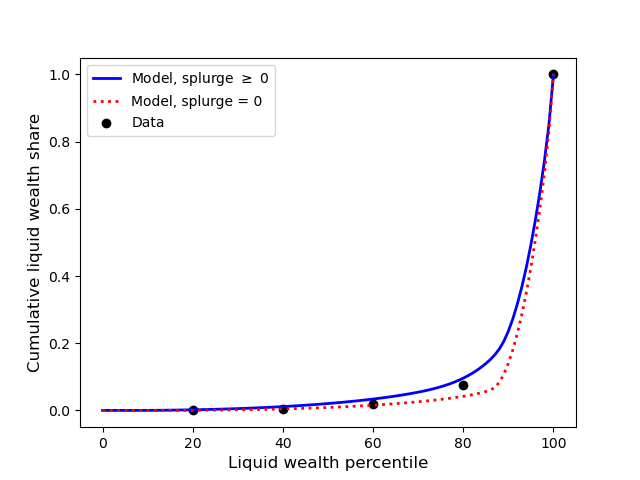
\includegraphics[width=\linewidth]{\econtexRoot/Code/HA-Models/Target_AggMPCX_LiquWealth/Figures/LiquWealth_Distribution_comparison_splurge0}
		\caption{Distribution of liquid wealth}
	\end{subfigure}%
	\caption{Marginal propensity to consume over time and the liquid wealth distribution in the model with and without the splurge as well as in the data}
	\notinsubfile{\label{fig:splurge0_Norwayestimation}}
	\parbox{16cm}{\small \vspace{.15cm} \textbf{Note}: Panel (a) shows the fit of the model to the dynamic consumption response estimated in {\citet{fagereng_mpc_2021}}; see their figure~A5.
Panel (b) shows the fit of the model to the distribution of liquid wealth (see Section~\ref{sec:SCFdata} for the definition) from the 2004 SCF.\normalsize}
\end{figure}


While the splurge helps in matching the empirical evidence on the iMPC, the model without the splurge also performs relatively well.
This is because the model without the splurge is able to generate a high initial marginal propensity to consume through a wider distribution of discount factors ($\beta = 0.921$ and $\nabla=0.116$) relative to the model with a splurge ($\beta = 0.968$ and $\nabla=0.0578$).
This ensures that sufficiently many agents are at the borrowing constraint and thus sensitive to transitory income shocks.\footnote{The model without the splurge implies there is a group of highly impatient households who have discount rates close to 0.8. While this is possible, such a discount rate implies these households care very little about their consumption even just a few years in the future.}

However, the model is not quite able to match the difference in spending between the initial year of the lottery win and the year after.
The model without the splurge exhibits a higher spending propensity in the year after the shock occurs as borrowing-constrained agents spend the additional income quicker.
The model without the splurge also provides a worse fit of the distribution of liquid wealth.
Relative to the baseline model, and to the data, the model without a splurge generates a more unequal wealth distribution.


The reason for these two effects, becomes apparent when considering the cross-sectional implications of the models with and without the splurge across different wealth quartiles.
While the model with the splurge can account for the empirically-observed initial MPCs among the wealthiest, the model without the splurge exhibits much lower MPCs among that group, see Table~\ref{tab:Comparison_Splurge_Table}.
The wealthiest group will thus be very patient and have low MPCs, which can explain why the wealth distribution becomes more unequal and doesn't quite fit the targeted distribution in the data in the version of the model without the splurge.


Overall, the model fit with the data deteriorates roughly by a factor of two measured by the Euclidean norm of the targeting error.\footnote{Specifically, the Euclidean norm of the targeting error increases from 0.04 to 0.08 for the time-profile of the marginal propensity to consume when the splurge is removed, from 0.16 to 0.29 for the marginal propensity to consume across wealth quartiles and from 0.027 to 0.032 for the Lorentz curve.} 

\begin{table}[t]
	\center
	\begin{tabular}{@{}lcccccc@{}} 
\toprule 
                  & \multicolumn{5}{c}{MPC} &   \\   
                  &  1st WQ  & 2nd WQ  & 3rd WQ & 4th WQ  & Agg  &  K/Y  \\  \midrule 
Splurge $\geq$ 0 &0.27 & 0.48 & 0.60 & 0.66 & 0.50 & 6.58 \\ 
Splurge = 0 &0.13 & 0.51 & 0.62 & 0.68 & 0.49 & 6.59 \\ 
Data &0.39 & 0.39 & 0.55 & 0.66 & 0.51 & 6.60 \\ 
\end{tabular}  

	\caption{Marginal propensities to consume across wealth quartiles and the total population as well as the wealth to income ratio, in the model with and without the splurge and according to the data}
	\notinsubfile{\label{tab:Comparison_Splurge_Table}}
\end{table}

\subsection{Estimating discount factor distributions without the splurge}

Figure~\ref{fig:LorenzPtsSplZero} shows that the model without splurge consumption can also match the wealth distributions in the three education groups very well.
We therefore turn to the implications of this version of the model for the untargeted moments discussed in section~\ref{sec:nonTargetedMoments}.


\begin{figure}[th]
	\begin{center}
		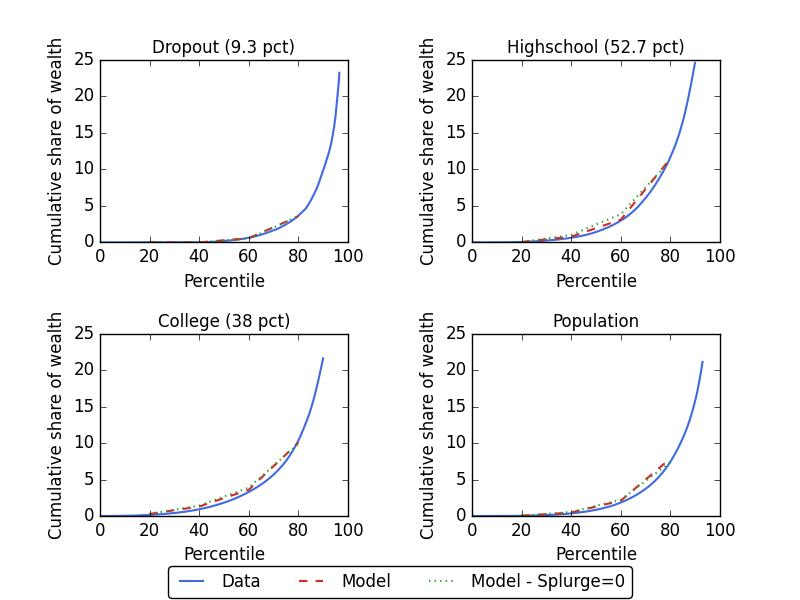
\includegraphics[width=.9\textwidth]{\econtexRoot/Figures/LorenzPoints_CRRA_2.0_R_1.01_wSplZero}
		\caption{Distributions of liquid wealth within each education group and for the whole population from the 2004 Survey of Consumer Finances and from the model estimated with and without splurge consumption}
		\notinsubfile{\label{fig:LorenzPtsSplZero}}
		\parbox{16cm}{\small \vspace{.15cm} \textbf{Note}: The discount factor distributions are estimated separately for each education group to fit the median liquid-wealth-to-permanent-income ratio and the $\nth{20}$, $\nth{40}$, $\nth{60}$, and $\nth{80}$ percentile points of the Lorenz curve for liquid wealth for that group. The ``Population'' panel compares the wealth distribution that results from pooling the three groups in the model to the overall wealth distribution in the data. The model is reestimated when the splurge is set to $0$.\normalsize}
		
	\end{center}
\end{figure}

The main difference between the models with and without splurge consumption is that without splurge consumption the MPCs drop for each education group and wealth quartile.
The difference is largest for the College group and for the highest wealth quartile (obviously with substantial overlap between these two groups).
This is shown in the two panels in Table~\ref{tab:nonTargetedMoments_wSplZero}.
The rest of the table shows that the distribution of wealth is not substantially different in the model estimated without splurge consumption.


\begin{table}[th]
	\begin{center}
		\begin{tabular}{l}
			\begin{tabular}{lcccc}
				\multicolumn{5}{l}{Panel (A) Non-targeted moments by education group} \\ \midrule
				& Dropout & Highschool & College & Population \\ \midrule
				Percent of liquid wealth (data) & 0.8 & 17.9 & 81.2 & 100 \\
				Percent of liquid wealth (model, baseline) & 1.2 & 20.1 & 78.7 & 100 \\
				Percent of liquid wealth (model, Splurge=0) & 1.6 & 18.7 & 79.7 & 100 \\
				\makecell[l]{Avg. lottery-win-year MPC \\ (model, incl. splurge)} & 0.78 & 0.63 & 0.44 & 0.54 \\ 
				\makecell[l]{Avg. lottery-win-year MPC \\ (model, splurge=0)} & 0.70 & 0.53 & 0.23 & 0.43
				\\ \bottomrule 
			\end{tabular} \\ \\ 
			
			\begin{tabular}{lcccc}
				\multicolumn{5}{l}{Panel (B) Non-targeted moments by wealth quartile} \\ \midrule
				& WQ 4 & WQ 3 & WQ 2 & WQ 1 \\ \midrule
				Percent of liquid wealth (data) & 0.14 & 1.60 & 8.51 & 89.76 \\
				Percent of liquid wealth (model, baseline) & 0.09 & 0.96 & 4.55 & 94.40 \\
				Percent of liquid wealth (model, Splurge=0) & 0.10 & 1.07 & 4.24 & 94.60 \\
				\makecell[l]{Avg. lottery-win-year MPC \\ (model, incl. splurge)} & 0.78 & 0.63 & 0.44 & 0.31 \\
				\makecell[l]{Avg. lottery-win-year MPC \\ (model, splurge=0)} & 0.69 & 0.53 & 0.36 & 0.14
				\\ \bottomrule 
			\end{tabular}
		\end{tabular}
		\caption{Model fit with respect to non-targeted moments}
		\notinsubfile{\label{tab:nonTargetedMoments_wSplZero}}
		\parbox{16cm}{\small \vspace{.15cm} \textbf{Note}: Panel (A) shows percent of liquid wealth held by each education group in the 2004 SCF and in the model.
It also shows the average MPCs after a lottery win for each education group.
The MPCs are calculated for each individual for the year of a lottery win, taking into account that the win takes place in a random quarter of the year that differs across individuals.
The MPCs are averaged across individuals within each education group.
Panel~(B) shows the same numbers for the population sorted into different quartiles of the liquid wealth distribution.\normalsize}
	\end{center}
\end{table}

%\begin{table}[th]
%	\begin{center}
%		\begin{tabular}{lccc}
%			\multicolumn{4}{l}{Model with Splurge=0} \\ \midrule
%			& Dropout & Highschool & College \\ \midrule
%			$(\beta_e, \nabla_e)$ & (0.700, 0.339) & (0.899, 0.106) & (0.978,0.019) \\
%			(Min, max) in approximation & (0.409, 0.991) & (0.809, $0.990$) & (0.962, 0.993) \\
%			\midrule 
%		\end{tabular}
%	\caption{Estimated discount factor distributions}
%		\notinsubfile{\label{tab:estimBetasSplZero}}
%		\parbox{16cm}{\small \vspace{.15cm} \textbf{Note}: Estimated parameters of the discount factor distributions for each education group in the model without splurge consumption. In parentheses are the minimum and maximum values we use in our discrete approximation to the uniform distribution of discount factors for each group. \normalsize}
%	\end{center}
%\end{table}

Finally, we again consider the  implications of our model for the dynamics of spending over time and for the dynamics of spending for households that remain unemployed long enough for unemployment benefits to expire.
Figure~\ref{fig:untargetedMoments_wSplZero} repeats Figure~\ref{fig:untargetedMoments} with results from the model without splurge consumption added.
The implication is that the model without a splurge leads to a slightly too low MPC in the year of a lottery win and a slightly higher MPC in the year after.


The drop in spending when unemployment benefits expire is virtually the same in the model without splurge consumption (17 percent versus 18 percent in the baseline).
While the consumption dynamics across the models with and without a splurge are fairly similar, the underlying drivers of the consumption drop upon expiry of unemployment benefits are different.
In the model with the splurge, the drop in income translates directly into lower consumption via the splurge itself.
In the model without the splurge it is the sharp rise in agents hitting the borrowing constraint which accounts for the consumption drop after UI benefits expire.
This is shown in the solid and dashed red lines in Figure~\ref{fig:expiryUI_wSplZero}, and is due to the wider distribution of discount factors that is needed to match the wealth distributions in the model without the splurge.
This leads to a greater number of agents being close the borrowing constraint.

\begin{figure}[thb]
	\centering
	\begin{subfigure}[b]{.48\linewidth}
		\centering
		\includegraphics[width=\linewidth]{\econtexRoot/Figures/iMPCs_both}
		\caption{Share of lottery win spent}
		\notinsubfile{\label{fig:USaggmpclotterywin_wSplZero}}
	\end{subfigure}
	\begin{subfigure}[b]{.48\linewidth}
		\centering
		\includegraphics[width=\linewidth]{\econtexRoot/Code/HA-Models/FromPandemicCode/Figures/Splurge0/UIextension_CompSplurge0}
		\caption{Spending upon expiry of UI benefits}
		\notinsubfile{\label{fig:expiryUI_wSplZero}}
	\end{subfigure}%
	\caption{Marginal propensity to consume over time and the spending upon expiry of UI benefits in the model}
	\notinsubfile{\label{fig:untargetedMoments_wSplZero}}
	\parbox{16cm}{\small \vspace{.15cm} \textbf{Note}: Panel (a) compares the dynamic consumption response in the model to the estimates in {\citet{fagereng_mpc_2021}}; see their Figure~A5.
Panel (b) shows the evolution of income and spending for households who remain unemployed long enough for UI benefits to expire; see Figure~2 in {\citet{ganongConsumer2019}}.\normalsize}
\end{figure}


%\begin{figure}[t]
%	\centering
%	\includegraphics[width=0.8\linewidth]{Code/HA-Models/FromPandemicCode/Figures/Splurge0/UIextension_CompSplurge0}
%	\caption{Consumption and income levels for agents staying unemployed for at least five quarters and the share of those agents at the borrowing limit, in the model with and without the splurge. Note: No policy nor the recession are active.}
%	\notinsubfile{\label{fig:UIextension_CompSplurge0}}
%\end{figure}


\FloatBarrier
\subsection{Multipliers in the absence of the splurge}

In this section we simulate the three fiscal policies from the main text in the estimated model without the splurge.
The shape of the impulse response functions only marginally change relative to the model with the splurge.
Hence, we focus on the quantitative changes as summarized by the cumulative multipliers in Figure \ref{fig:cumulativemultipliers_SplurgeComp}.
The figure shows the multipliers when AD effects are switched on for the model with and without the splurge.
Table \ref{tab:Multiplier_SplurgeComp} shows the 10y-horizon multiplier across the two models.

The absence of the splurge entails a calibration with a lower average MPC in the population.
Hence, the check and tax cut exhibit lower multipliers when there is no splurge.
For the UI extension we observe the opposite pattern, as the multiplier is larger in the model without the splurge.
This due to the consumption dynamics around the expiry of UI benefits described in the previous section.
In the model without the splurge more agents hit the borrowing constraint upon the expiry of benefits.
Providing those agents with an extension of UI benefits thus turns out to be slightly more powerful.


The policy ranking in terms of the multiplier shifts slighlty.
In the model with the splurge, the check policy delivers multiplier effects much more rapidly than the UI extension.
In the model without splurge consumption, the UI extension appears superior to the check, both at shorter and longer horizons.
Both models agree on the tax cut being the least effective policy.


\begin{figure}[t]
	\centering
	\caption{Cumulative multiplier as a function of the horizon for the three policies with and without the splurge. Note: Policies are implemented during a recession with AD effect active.}
	\notinsubfile{\label{fig:cumulativemultipliers_SplurgeComp}}
\end{figure}


\begin{table}[t]
	\center
	\begin{tabular}{@{}lccc@{}} 
\toprule 
& Stimulus check    & UI extension    & Tax cut     \\  \midrule 
10y-horizon Multiplier (no AD effect)  &0.870(0.879)  & 0.910(0.906)  & 0.839(0.847)     \\ 
10y-horizon Multiplier (AD effect) &1.143(1.234)  & 1.221(1.211)  & 0.947(0.978)     \\ 
\end{tabular}  
tabular}  

	\caption{Multipliers, calculated for policies implemented in a recession with and without aggregate demand effects. }
	\parbox{16cm}{\small \vspace{.15cm} \textbf{Note}: The values outside of the brackets capture the multipliers in the model without the splurge, while those inside the brackets are the corresponding mulitipliers with the splurge. \normalsize}
	\notinsubfile{\label{tab:Multiplier_SplurgeComp}}
\end{table}





%\subfile{Robustness}
\subfile{\econtexRoot/Subfiles/Appendix-HANK}

\ifthenelse{\boolean{Web}}{}{
\end{document} \endinput
}

